% Options for packages loaded elsewhere
\PassOptionsToPackage{unicode}{hyperref}
\PassOptionsToPackage{hyphens}{url}
\documentclass[
  11pt,
]{article}
\usepackage{xcolor}
\usepackage[margin=22mm]{geometry}
\usepackage{amsmath,amssymb}
\setcounter{secnumdepth}{-\maxdimen} % remove section numbering
\usepackage{iftex}
\ifPDFTeX
  \usepackage[T1]{fontenc}
  \usepackage[utf8]{inputenc}
  \usepackage{textcomp} % provide euro and other symbols
\else % if luatex or xetex
  \usepackage{unicode-math} % this also loads fontspec
  \defaultfontfeatures{Scale=MatchLowercase}
  \defaultfontfeatures[\rmfamily]{Ligatures=TeX,Scale=1}
\fi
\usepackage{lmodern}
\ifPDFTeX\else
  % xetex/luatex font selection
\fi
% Use upquote if available, for straight quotes in verbatim environments
\IfFileExists{upquote.sty}{\usepackage{upquote}}{}
\IfFileExists{microtype.sty}{% use microtype if available
  \usepackage[]{microtype}
  \UseMicrotypeSet[protrusion]{basicmath} % disable protrusion for tt fonts
}{}
\makeatletter
\@ifundefined{KOMAClassName}{% if non-KOMA class
  \IfFileExists{parskip.sty}{%
    \usepackage{parskip}
  }{% else
    \setlength{\parindent}{0pt}
    \setlength{\parskip}{6pt plus 2pt minus 1pt}}
}{% if KOMA class
  \KOMAoptions{parskip=half}}
\makeatother
\setlength{\emergencystretch}{3em} % prevent overfull lines
\providecommand{\tightlist}{%
  \setlength{\itemsep}{0pt}\setlength{\parskip}{0pt}}
\usepackage{bookmark}
\IfFileExists{xurl.sty}{\usepackage{xurl}}{} % add URL line breaks if available
\urlstyle{same}
\hypersetup{
  hidelinks,
  pdfcreator={LaTeX via pandoc}}

\author{}
\date{}

\usepackage{graphicx}
\begin{document}

\section{The two graph-domain quotients of the local
inverse}\label{the-two-graph-domain-quotients-of-the-local-inverse}

This editorial note derives the graph-domain consequences of the
completed local inverse. Its receiving proofs are
\href{https://github.com/KokunoYumeto/open-math-courses/blob/b1f73325069d9568d9acb6e27036b1b0f4cad7fd/docs/courses/elliptic-operators-and-boundary-problems/src/local-elliptic-coefficients.md\#L1846}{Section
14.6, (CS40)--(CS50)} and
\href{https://github.com/KokunoYumeto/open-math-courses/blob/b1f73325069d9568d9acb6e27036b1b0f4cad7fd/docs/courses/elliptic-operators-and-boundary-problems/src/local-elliptic-coefficients.md\#L2213}{the
unchanged example in Section 14.8.5, (CE25)--(CE34)}. The original
lesson construction and the unchanged example remain explicit
throughout. These source links require access to the course repository.
The complete packaged proofs are
\href{../../local-elliptic-coefficients.html\#eq-CS40}{the local inverse
identities} and
\href{../../local-elliptic-coefficients.html\#eq-CE25}{the
original-coefficient example}.

All spaces below are complex. The \(L^2\) inner
product is linear in its first argument. Distribution pairings retain
the complex-bilinear convention of U006. The Hilbert adjoint introduced
below consequently involves conjugation; it is a different operation
from the distributional transpose \(p(D)\mapsto p(-D)\) in U006
(CS4).

\subsection{1. The unchanged polynomial graph space and completed
maps}\label{the-unchanged-polynomial-graph-space-and-completed-maps}

Retain the original nonzero polynomial \(p\in\mathbb C[\xi_1,\ldots,\xi_n]\), its
degree \(m\), the original coordinates, and
\(D_j=-i\partial_{x_j}\). For every polynomial
\(q\), keep the full strength array

\[
 \widetilde q(\xi)^2=\sum_{\alpha\in\mathbb N^n}|\partial_\xi^\alpha q(\xi)|^2,
 \qquad
 V_p=\{q:\widetilde q(\xi)\leq C_q\widetilde p(\xi)
       \text{ for every }\xi\in\mathbb R^n\text{ and some finite }C_q\},
 \qquad
 \|q\|_p=\sup_{\xi\in\mathbb R^n}\frac{\widetilde q(\xi)}{\widetilde p(\xi)}.
 \tag{GM1}
\]

Every zeroth and higher derivative, including its zero value, remains
part of this definition. To recall why its denominator is positive,
choose a nonzero degree-\(m\) coefficient
\(a_{\alpha_0}\). Then \(\partial^{\alpha_0}p=\alpha_0!a_{\alpha_0}\), so
\(\widetilde p\geq\alpha_0!|a_{\alpha_0}|>0\). For \(m=0\), this bound
is \(|p|>0\). It follows that
\(1,p\in V_p\), with \(\|p\|_p=1\). The
pointwise triangle inequality for the complete derivative arrays makes
\(V_p\) a vector space and \(\|\cdot\|_p\)
a norm.

This vector space is finite dimensional. Indeed
\(\widetilde p(\xi)\leq A(1+|\xi|)^m\) for some finite \(A\),
since its derivative array is finite and each entry is a polynomial of
degree at most \(m\). If \(q\in V_p\)
had degree \(d>m\), its
degree-\(d\) part would be nonzero at some real
vector \(v\). A polynomial zero on every real
vector has every coefficient zero: apply the one-variable root bound in
the first variable for each fixed choice of the other variables and
repeat by induction. Consequently \(q(tv)=t^d q_d(v)+O(t^{d-1})\) would
contradict \(|q(tv)|\leq\|q\|_p A(1+t|v|)^m\). Thus \(V_p\)
lies in the finite-dimensional space of polynomials of degree at most
\(m\). These are also the arguments in U006
(CS5)--(CS6).

Choose the actual basis \(q_1,\ldots,q_s\) used for the graph
norm. Retain the original polynomials \(p_\nu\in V_p\),
coefficients \(c_\nu\in C(\Omega)\) with \(c_\nu(x_0)=0\),
and the bounded open neighborhood \(U\) of (CS42).
In particular the coefficients are bounded on
\(U\), because \(\overline U\subset\Omega\) is
compact. Put \(Y=L^2(U)\), and use exactly the full common
maximal graph space

\[
 H=\mathcal H_p(U)=\{u\in L^2(U):q_j(D)u\in L^2(U),\ 1\leq j\leq s\},
 \qquad
 \|u\|_H^2=\|u\|_2^2+\sum_{j=1}^s\|q_j(D)u\|_2^2.
 \tag{GM2}
\]

The derivatives in this definition are distributional. Its inner product
is the corresponding sum of the original \(L^2\)
inner products. Completeness follows directly: if
\(u_k\) is Cauchy in this norm, let
\(u\) and \(v_j\) be the
\(L^2\) limits of \(u_k\) and
\(q_j(D)u_k\). Testing against a compactly supported smooth
function shows \(q_j(D)u=v_j\), because differentiation is
continuous in the distributional topology and \(L^2\)
convergence implies distributional convergence by Cauchy--Schwarz. Thus
\(u\in H\) and \(u_k\to u\) in
\(H\). A basis expansion proves that the set
\(H\) contains the \(L^2\)
distributional derivative for every \(q\in V_p\). No graph
norm is changed when this fact is used.

Write the exact basis expansions

\[
 p=\sum_{j=1}^s\alpha_jq_j,
 \qquad p_\nu=\sum_{j=1}^s\beta_{\nu j}q_j,
 \qquad
 g_j(x)=\alpha_j+\sum_{\nu=1}^r c_\nu(x)\beta_{\nu j}.
 \tag{GM3}
\]

The graph-domain realization of the original operator is

\[
 P:H\longrightarrow Y,
 \qquad
 Pu=p(D)u+\sum_{\nu=1}^r c_\nu p_\nu(D)u
    =\sum_{j=1}^s g_jq_j(D)u.
 \tag{GM4}
\]

Every coefficient multiplies an already defined
\(L^2\) function. Define the finite bound

\[
 C_P=\mathop{\rm ess\,sup}_{x\in U}
           \left(\sum_{j=1}^s|g_j(x)|^2\right)^{1/2}.
 \tag{GM5}
\]

Pointwise Cauchy--Schwarz followed by integration proves
\(\|Pu\|_2\leq C_P\|u\|_H\). This is an explicit bound, with every
original coefficient present; sharpness of the operator norm is not
claimed.

Keep the completed maps \(S_U,B_U,T_U^{-1}\), and
\(E=S_UT_U^{-1}\) from (CS38)--(CS50), rather than constructing
a new inverse. Keep

\[
 K_0=K_{m,n,R_0},\qquad
 b=K_0\sum_{\nu=1}^r\|p_\nu\|_p\sup_U|c_\nu|<1,
 \qquad
 C_E=\frac{K_0}{1-b}
       \left(\|1\|_p^2+\sum_{j=1}^s\|q_j\|_p^2\right)^{1/2}.
 \tag{GM6}
\]

Equations (CS41), (CS45), and (CS47) give the bounded map
\(E:Y\to H\) with \(\|Ef\|_H\leq C_E\|f\|_2\). Equation
(CS48) proves \(PE=I_Y\); equation (CS50) proves
\(EPu=u\) for \(u\in C_c^\infty(U)\). These are
completed input results, with their full proofs retained in the input
lesson. This note derives their domain consequences without adding a
solvability premise or suppressing any part of their construction.

\subsection{2. The minimal domain, its closed image, and the exact
kernel
projection}\label{the-minimal-domain-its-closed-image-and-the-exact-kernel-projection}

Define the actual minimal common graph domain by

\[
 H_{\min}=\overline{C_c^\infty(U)}^{\|\cdot\|_H},
 \qquad M=P(H_{\min})\subset Y,
 \qquad N=\ker(P:H\to Y).
 \tag{GM7}
\]

\textbf{Theorem GM-A.} The identity \(EP=I\) holds on
\(H_{\min}\). The restriction \(P_{\min}:H_{\min}\to M\)
is a bounded bijection with inverse \(E|_M\), and

\[
 \|u\|_H\leq C_E\|Pu\|_2\quad(u\in H_{\min}),
 \qquad E(M)=H_{\min},
 \qquad N\cap H_{\min}=\{0\}.
 \tag{GM8}
\]

The image \(M\) is closed in
\(Y\). The exact operator

\[
 Q=I_H-EP:H\to H
 \tag{GM9}
\]

is a bounded projection onto \(N\), with kernel
\(E(Y)\), and

\[
 Q^2=Q,\quad PQ=0,\quad QE=0,\quad Q|_N=I_N,\quad
 \|Q\|_{H\to H}\leq 1+C_EC_P.
 \tag{GM10}
\]

It vanishes on \(H_{\min}\). The completed solution space
is the exact topological direct sum

\[
 H=N\mathbin{\dotplus}E(Y),\qquad
 u=Qu+E(Pu).
 \tag{GM11}
\]

For every \(f\in Y\), all solutions in this original
graph domain, and only those solutions, are

\[
 \{u\in H:Pu=f\}=Ef+N.
 \tag{GM12}
\]

\emph{Proof.} For \(u\in H_{\min}\), choose
\(u_k\in C_c^\infty(U)\) with \(u_k\to u\) in
\(H\). Boundedness of \(P\)
gives \(Pu_k\to Pu\) in \(Y\).
Boundedness of \(E:Y\to H\) then gives
\(EPu_k\to EPu\) in \(H\). On the
compactly supported functions the input identity
\(EPu_k=u_k\) is initially an equality in
\(L^2\), and hence an equality in
\(H\), since the equal \(L^2\)
classes have the same distributional derivatives. Taking the limit
proves \(EPu=u\) in \(H\). The
estimate in (GM8) follows. It proves injectivity of
\(P_{\min}\); surjectivity onto \(M\)
is its definition. If \(f=Pu\in M\) with
\(u\in H_{\min}\), then \(Ef=u\in H_{\min}\). Conversely
\(u=E(Pu)\) for every \(u\in H_{\min}\). Thus
\(E(M)=H_{\min}\), and \(N\cap H_{\min}=0\).

To prove closedness, let \(f_k\in M\) converge in
\(Y\) to \(f\). Write
\(u_k=Ef_k\in H_{\min}\). The bound for \(E\)
gives \(u_k\to Ef\) in \(H\). Since
\(H_{\min}\) is closed, \(Ef\in H_{\min}\); since
\(PEf=f\), it follows that \(f\in M\).
This proves the claimed closedness without a Fredholm or ellipticity
assumption.

The identity \(PE=I_Y\) gives
\((EP)^2=EP\). Expanding \((I-EP)^2\) proves
\(Q^2=Q\). It also gives \(PQ=P-PEP=0\) and
\(QE=E-EPE=0\). If \(v\in N\), then
\(Qv=v\), so the range of \(Q\)
is exactly \(N\). If \(Qu=0\),
then \(u=E(Pu)\in E(Y)\); if \(u=Ef\), then
\(Qu=0\). Thus the kernel is exactly
\(E(Y)\). Both summands are closed:
\(N\) is the kernel of a bounded map, and
\(E(Y)\) is the kernel of \(Q\).
The intersection is zero, because \(PEf=0\) implies
\(f=0\). Formula (GM11) is the definition of
\(Q\). Its projections are
\(Q\) and \(EP\), so the direct
sum is topological. The norm bound in (GM10) is the triangle inequality
and the two operator bounds. Finally \(P(Ef+v)=f\) for
\(v\in N\); any solution \(u\)
satisfies \(P(u-Ef)=0\). This proves (GM12).
\hfill\ensuremath{\blacksquare}

\textbf{Corollary GM-A1: the single-operator minimal closure.} Consider
\(P\) on \(C_c^\infty(U)\subset L^2(U)\) with its
original expression (GM4). Its closure as an unbounded operator in
\(L^2(U)\) has domain exactly
\(H_{\min}\), and it is injective with closed range
\(M\). On this domain the original full graph norm
and the single-operator graph norm obey

\[
 \|u\|_H\leq C_E\left(\|u\|_2^2+\|Pu\|_2^2\right)^{1/2},
 \qquad
 \left(\|u\|_2^2+\|Pu\|_2^2\right)^{1/2}
       \leq (1+C_P^2)^{1/2}\|u\|_H.
 \tag{GM13}
\]

\emph{Proof.} The second estimate holds on all of
\(H\) by (GM2) and (GM5); the first follows from
(GM8). If \(u_k\in C_c^\infty(U)\) converges in the single-operator
graph norm, the difference version of (GM8) makes it Cauchy in the full
original \(H\) norm. Its \(H\)
limit is in \(H_{\min}\) and agrees with its
\(L^2\) limit, and boundedness of
\(P\) identifies the limiting image. Conversely the
defining \(H\)-approximation for
\(H_{\min}\) gives approximation in the single-operator
graph norm by the second estimate. This proves equality of the two
closures while retaining both norms and their exact comparison.

For closedness as an unbounded operator, suppose
\(u_k\in H_{\min}\), \(u_k\to u\) in
\(L^2\), and \(Pu_k\to f\) in
\(L^2\). Again (GM8) makes \(u_k\)
Cauchy in \(H\). Its limit belongs to
\(H_{\min}\), agrees with \(u\), and
has image \(f\). The domain is dense in
\(L^2(U)\), because it contains
\(C_c^\infty(U)\), which is dense: truncate an
\(L^2\) function to compact subsets a positive
distance from the boundary, then mollify with radii smaller than that
distance. The truncations converge by dominated convergence, and the
mollifications by translation continuity in \(L^2\).
These operations are also proved in the prerequisite cited in U006
before (CS38). Injectivity and closed range were proved in GM-A.
\hfill\ensuremath{\blacksquare}

The word ``maximal'' in (GM2) refers to all original constant-polynomial
derivatives in \(V_p\). We have not replaced that
domain by a domain that asks only for \(Pu\in L^2\). For
continuous coefficients, multiplying an arbitrary distributional
derivative by a coefficient is not automatically defined. The exact
closure statement just proved applies to the minimal operator and
supplies the bridge between its two graph norms without altering the
maximal common domain.

\subsection{3. The complete quotient maps, constants, and three
projections}\label{the-complete-quotient-maps-constants-and-three-projections}

Equip \(H/H_{\min}\) and \(Y/M\) with
their actual quotient norms:

\[
 \|[u]\|_{H/H_{\min}}=\inf_{h\in H_{\min}}\|u-h\|_H,
 \qquad
 \|[f]\|_{Y/M}=\inf_{m\in M}\|f-m\|_2.
 \tag{GM14}
\]

On \(N\oplus(Y/M)\), use the Hilbert direct-sum norm

\[
 \|(v,[f])\|_\oplus^2=\|v\|_H^2+\|[f]\|_{Y/M}^2.
 \tag{GM15}
\]

\textbf{Theorem GM-B.} The following explicit maps are inverse bounded
linear isomorphisms:

\[
 \Phi:H/H_{\min}\longrightarrow N\oplus(Y/M),
 \qquad \Phi([u])=(Qu,[Pu]),
 \tag{GM16}
\]

\[
 \Psi:N\oplus(Y/M)\longrightarrow H/H_{\min},
 \qquad \Psi(v,[f])=[v+Ef].
 \tag{GM17}
\]

Put \(C_Q=1+C_EC_P\). Their original-norm bounds are

\[
 \|\Phi\|\leq(C_Q^2+C_P^2)^{1/2},
 \qquad
 \|\Psi\|\leq(1+C_E^2)^{1/2}.
 \tag{GM18}
\]

The exact quotient norm, before using either estimate, is

\[
 \|\Psi(v,[f])\|_{H/H_{\min}}
       =\inf_{m\in M}\|v+E(f-m)\|_H.
 \tag{GM19}
\]

There is also the split exact sequence with all original connecting maps

\[
 0\longrightarrow N
 \xrightarrow{v\mapsto[v]}H/H_{\min}
 \xrightarrow{[u]\mapsto[Pu]}Y/M
 \longrightarrow0,
 \qquad [f]\mapsto[Ef]
 \text{ is a bounded splitting.}
 \tag{GM20}
\]

\emph{Proof.} If \(u\) is replaced by
\(u+h\) for \(h\in H_{\min}\), then
\(Qh=0\) and \(Ph\in M\), so (GM16) is
well defined. If \(f\) is replaced by
\(f+m\) for \(m\in M\), then
\(Em\in H_{\min}\), so (GM17) is well defined. Using
\(QE=0\), \(Qv=v\),
\(Pv=0\), and \(PEf=f\), we obtain
\(\Phi\Psi(v,[f])=(v,[f])\). Using (GM11), we obtain
\(\Psi\Phi([u])=[Qu+EPu]=[u]\).

For every \(h\in H_{\min}\), \[
 \|Qu\|_H\leq C_Q\|u-h\|_H,
 \qquad \|[Pu]\|_{Y/M}\leq\|P(u-h)\|_2\leq C_P\|u-h\|_H.
\] Square,
add, and take the infimum to obtain the first bound. For every
\(m\in M\), \[
 \|[v+Ef]\|_{H/H_{\min}}
  \leq\|v+E(f-m)\|_H
  \leq\|v\|_H+C_E\|f-m\|_2.
\] Taking the
infimum and then applying two-variable Cauchy--Schwarz proves the second
bound. Since \(H_{\min}=E(M)\), the infimum in the definition
of the quotient norm is exactly (GM19), not a newly imposed norm. The
injection in (GM20) is injective because \(N\cap H_{\min}=0\). The
second map is surjective because \(PE=I\). If
\([Pu]=0\), then \(Pu\in M\), so
\(EPu\in H_{\min}\) and \([u]=[Qu]\) is in the
displayed injection. The splitting follows from
\(PE=I\) and is bounded by \(C_E\).
Thus every assertion of exactness and splitting is established.
\hfill\ensuremath{\blacksquare}

For completeness, a closed subspace \(M\) of a
Hilbert space has an orthogonal projection with norm at most one. Here
is the argument used below. For \(f\in Y\), let
\(d=\inf_{m\in M}\|f-m\|_2\), and choose \(m_k\in M\)
approaching that infimum. The parallelogram identity gives
\[
 \|m_k-m_\ell\|_2^2
 \leq 2\|f-m_k\|_2^2+2\|f-m_\ell\|_2^2-4d^2\longrightarrow0.
\] Thus \(m_k\to m\in M\). The real
one-variable variation of \(\|f-m-tz\|^2\), first for
\(z\in M\), then for \(iz\), proves
\(f-m\perp M\). This orthogonal decomposition is unique,
depends linearly on \(f\), and its two squared
component norms add to \(\|f\|_2^2\); consequently each
projection has norm at most one. Write these projections as
\(\Pi_M\) and \(\Pi_{M^\perp}\).

There are three actual bounded projections on
\(H\):

\[
 Q=I-EP,
 \qquad R_{\min}=E\Pi_M P,
 \qquad R_{\perp}=E\Pi_{M^\perp}P.
 \tag{GM21}
\]

Their ranges are respectively \(N,H_{\min},E(M^\perp)\), their pairwise
products in both orders are zero, and their sum is
\(I_H\). Indeed \(PE=I\), the two
orthogonal \(Y\)-projections square to themselves
and have zero products, and \(PQ=QE=0\). The range of
\(R_{\min}\) is \(E(M)=H_{\min}\), and it is the
identity there because \(EP=I\) on that domain. The
same calculation proves the other range and identity. Thus

\[
 H=H_{\min}\mathbin{\dotplus}N\mathbin{\dotplus}E(M^\perp),
 \qquad
 \|R_{\min}\|,\|R_{\perp}\|\leq C_EC_P.
 \tag{GM22}
\]

These sums use the original \(H\) norm.
Orthogonality between their \(H\)-summands is not
asserted. The precise quotient-coordinate map is also
\([u]\mapsto(Qu,\Pi_{M^\perp}Pu)\), because \([f]\mapsto\Pi_{M^\perp}f\) is an
isometry from \(Y/M\) onto
\(M^\perp\).

\subsection{4. The second factor is the exact adjoint obstruction
space}\label{the-second-factor-is-the-exact-adjoint-obstruction-space}

Define the original Hilbert formal adjoint distribution on
\(v\in L^2(U)\) by

\[
 P^\dagger v
   =\overline p(D)v
       +\sum_{\nu=1}^r\overline{p_\nu}(D)
                           (\overline{c_\nu}\,v),
 \qquad
 N^\dagger=\{v\in L^2(U):P^\dagger v=0\text{ in }\mathcal D'(U)\}.
 \tag{GM23}
\]

The bars on polynomials conjugate their coefficients, not their
variables. Each product inside a derivative is an
\(L^2\) function; distributional differentiation of
that product is defined even when \(c_\nu\) is only
continuous. No derivative of a continuous coefficient is postulated as a
function.

\textbf{Theorem GM-C.} One has \(M^\perp=N^\dagger\). In particular
the quotient factor \(Y/M\) is isometrically
isomorphic to the exact distributional adjoint kernel, and the original
full graph-domain quotient has the bounded isomorphism

\[
 H/H_{\min}\longrightarrow N\oplus N^\dagger,
 \qquad [u]\longmapsto(Qu,\Pi_{N^\dagger}Pu),
 \qquad
 (v,w)\longmapsto[v+Ew]
 \tag{GM24}
\]

with the bounds in (GM18), using the \(H\) norm on
\(N\) and the \(L^2\) norm on
\(N^\dagger\).

\emph{Proof.} For \(u\in C_c^\infty(U)\), integration by parts or
the definition of distributional derivatives gives

\[
 \langle Pu,v\rangle_{L^2}
   =\overline{\langle P^\dagger v,\overline u\rangle_{\mathcal D',\mathcal D}}.
 \tag{GM25}
\]

For the signs, \(D_j=-i\partial_j\), its distributional transpose
is \(-D_j\), and \(-D_j\overline u=\overline{D_ju}\). The same
identity term by term in the complete polynomials gives
\(\overline p(D)\) on \(v\) and
\(\overline{p_\nu}(D)\) on \(\overline{c_\nu}v\). There is no
boundary contribution because \(u\) is compactly
supported.

If \(v\perp M\), its pairing with
\(Pu\) vanishes for every such
\(u\), so (GM25) proves \(P^\dagger v=0\).
Conversely, if \(P^\dagger v=0\), the pairing vanishes on
\(C_c^\infty(U)\). For any \(u\in H_{\min}\), choose
the original graph approximation \(u_k\to u\). Then
\(Pu_k\to Pu\) in \(L^2\), so
Cauchy--Schwarz extends the zero pairing to \(Pu\).
Hence \(v\perp M\). This proves equality. Since
\(M\) is closed, the orthogonal quotient
identification proved after GM-B applies. Substitution in (GM16)--(GM17)
gives (GM24) and its inverse, and all bounds are unchanged.
\hfill\ensuremath{\blacksquare}

The unbounded adjoint of the closed densely defined minimal operator of
GM-A1 has the complete domain

\[
 \operatorname{Dom}(P_{\min}^*)
   =\{v\in L^2(U):P^\dagger v\in L^2(U)\text{ as a distribution}\},
 \qquad P_{\min}^*v=P^\dagger v.
 \tag{GM26}
\]

To prove this, the defining adjoint equality on
\(H_{\min}\) restricts to (GM25), and so identifies its
representing \(L^2\) function with
\(P^\dagger v\). Conversely an \(L^2\)
representing function for \(P^\dagger v\) gives the adjoint
equality first on the compactly supported functions by (GM25), then on
\(H_{\min}\) by graph approximation; both
\(u_k\to u\) and \(Pu_k\to Pu\) in
\(L^2\). This proves both inclusions of the domain
and the displayed operator formula. Therefore the space
\(N^\dagger\) in (GM24) is exactly
\(\ker P_{\min}^*\), with no additional regularity condition.

There is an exact existence criterion for the minimal-domain solution:
for \(f\in Y\), a solution \(u\in H_{\min}\) of
\(Pu=f\) exists if and only if
\(\langle f,v\rangle_2=0\) for every \(v\in N^\dagger\). In that
event its unique value is \(u=Ef\). Indeed a
minimal-domain image lies in \(M\) and is
orthogonal to \(M^\perp=N^\dagger\). Conversely the orthogonal
decomposition \(f=\Pi_Mf+\Pi_{M^\perp}f\), proved above, shows that
orthogonality to \(M^\perp\) forces the second component
to vanish, so \(f\in M\). Equation (GM8) then puts
\(Ef\) in \(H_{\min}\), and
\(PEf=f\). Injectivity of \(P_{\min}\)
proves uniqueness. Thus the second quotient factor specifies the exact
right-hand-side obstruction and its receiving map, while the first
specifies the ambiguity among full graph-domain solutions.

\subsection{5. The unchanged example and its entire kernel
modes}\label{the-unchanged-example-and-its-entire-kernel-modes}

Now retain every quantity of U006 (CE1)--(CE34):

\[
 p(\xi_1,\xi_2)=\xi_1^2+i\xi_2,
 \qquad n=2,\quad m=2,\quad x_0=(0,0),
 \qquad U=(-1/4,1/4)^2,
 \tag{GM27}
\]

\[
 \widetilde p(\xi)^2
   =|\xi_1^2+i\xi_2|^2+|2\xi_1|^2+|i|^2+|2|^2
   =\xi_1^4+\xi_2^2+4\xi_1^2+1+4,
 \tag{GM28}
\]

\[
 C=\begin{pmatrix}14&-20&7\\-20&32&-12\\7&-12&5\end{pmatrix},
 \quad\lambda_*=\text{the largest eigenvalue of }C,
 \quad K=41472\lambda_*\sqrt{33}\,e^2,
 \quad a=\sqrt{\frac{\sqrt2-1}{2}},
 \quad\varepsilon=\frac2{Ka}>0,
 \quad c(x)=\varepsilon x_1.
 \tag{GM29}
\]

Here \(\lambda_*\) is the matrix eigenvalue from U006
(CE7)--(CE10). It is not the freely varying mode parameter
\(\lambda\) below. The full original differential
expression becomes

\[
 P=D_1^2+iD_2+\varepsilon x_1D_1
  =-\partial_1^2+\partial_2-i\varepsilon x_1\partial_1.
 \tag{GM30}
\]

Indeed \((-i)^2=-1\), \(i(-i)=1\), and
\(\varepsilon x_1(-i)=-i\varepsilon x_1\). Thus every sign and the nonzero drift
coefficient are retained.

\textbf{Lemma GM-D1: the full weaker-polynomial space.} For this actual
\(p\),

\[
 V_p=\operatorname{span}_{\mathbb C}\{1,\xi_1,\xi_1^2,\xi_2\},
 \quad
 \|1\|_p=1/\sqrt5,
 \quad\|\xi_1\|_p=a,
 \quad\|\xi_1^2\|_p=1,
 \quad\|\xi_2\|_p=1.
 \tag{GM31}
\]

\emph{Proof.} The degree argument after (GM1) puts every
\(q\in V_p\) in degree at most two. Write its complete
expression \[
 q=A_{20}\xi_1^2+A_{11}\xi_1\xi_2+A_{02}\xi_2^2
       +A_{10}\xi_1+A_{01}\xi_2+A_{00}.
\] At \((0,t)\), the
bound \(|q(0,t)|\leq C_q\sqrt{t^2+1+4}\) forces \(A_{02}=0\) by
dividing by \(t^2\) and taking
\(t\to+\infty\). At \((t,t^2)\), the complete
denominator is \(\sqrt{t^4+t^4+4t^2+1+4}\); dividing the bound by
\(t^3\) then forces \(A_{11}=0\). All
remaining coefficients are unrestricted once the four displayed
monomials are in \(V_p\).

For \(1\), the complete strength numerator is
\(1\), whose ratio is maximal at
\((0,0)\), where the denominator is
\(\sqrt{1+4}=\sqrt5\). For \(\xi_1\), the squared
ratio is \[
 \frac{\xi_1^2+1}{\xi_1^4+\xi_2^2+4\xi_1^2+1+4}.
\] It is maximal at
\(\xi_2=0\). Put \(t=\xi_1^2\geq0\).
Differentiating \((t+1)/(t^2+4t+1+4)\) gives numerator
\(-t^2-2t+1\); it is positive before
\(t=\sqrt2-1\) and negative afterwards. Substitution gives
\((\sqrt2-1)/2=a^2\), including the actual endpoint value
\(1/5\) and the limit \(0\). For
\(\xi_1^2\), the squared ratio is
\[
 \frac{\xi_1^4+4\xi_1^2+4}{\xi_1^4+\xi_2^2+4\xi_1^2+1+4}\leq1,
\] and its values at \((t,0)\)
tend to one. For \(\xi_2\), the squared ratio is
\[
 \frac{\xi_2^2+1}{\xi_1^4+\xi_2^2+4\xi_1^2+1+4}\leq1,
\] and its values at \((0,t)\)
tend to one. Thus the two suprema are exactly one. The derivative-array
triangle inequality shows that every linear combination of these four
monomials is in \(V_p\); their polynomial
independence makes them a basis. \hfill\ensuremath{\blacksquare}

For the explicit norm calculation choose the basis
\((1,\xi_1,\xi_1^2,\xi_2)\). This is a declared instance of the basis in
(GM2), not a replacement of \(p\). The graph set
and its full norm are

\[
 H=\{u\in L^2(U):D_1u,D_1^2u,D_2u\in L^2(U)\},
 \quad
 \|u\|_H^2=\|u\|_2^2+\|u\|_2^2
                    +\|D_1u\|_2^2+\|D_1^2u\|_2^2+\|D_2u\|_2^2.
 \tag{GM32}
\]

In this exact basis the full coefficient vector of
\(P\) is \((0,\varepsilon x_1,1,i)\). Hence

\[
 C_P=\left(|0|^2+\varepsilon^2/16+|1|^2+|i|^2\right)^{1/2},
 \qquad
 b=Ka\sup_U|c|=Ka\frac{\varepsilon}{4}=\frac12,
 \quad
 C_E=2K\left(\frac15+\frac15+a^2+1+1\right)^{1/2}.
 \tag{GM33}
\]

The supremum for \(C_P\) is the essential supremum
over the unchanged open square; values approach its endpoints on sets of
positive measure. The two \(1/5\) terms in
\(C_E\) are respectively the separate
\(\|1\|_p^2\) term of the graph estimate and the
\(q_1=1\) contribution. The two
\(1\) terms belong to \(\xi_1^2\)
and \(\xi_2\). None is absorbed or omitted. Thus all
results GM-A--GM-C apply with the constants (GM29) and (GM33).

\textbf{Theorem GM-D2: the requested even modes.} For every
\(\lambda\in\mathbb C\), put the empty product equal to one and
define

\[
 c_k(\lambda)=\frac{\prod_{h=0}^{k-1}(\lambda-2i\varepsilon h)}{(2k)!},
 \qquad
 \varphi_\lambda(z)=\sum_{k=0}^\infty c_k(\lambda)z^{2k},
 \qquad
 u_\lambda(x_1,x_2)=e^{\lambda x_2}\varphi_\lambda(x_1).
 \tag{GM34}
\]

The series and every derivative converge uniformly on every compact
subset of \(\mathbb C^2\). The functions are entire, lie in
the full actual space \(H\), and satisfy
\(Pu_\lambda=0\). Any finite family with distinct parameters
is linearly independent. In particular \(N\) and
\(H/H_{\min}\) are infinite dimensional, and every
\(u_\lambda\) represents a nonzero class in
\(H/H_{\min}\).

\emph{Proof of convergence and derivatives.} Put
\(A_\lambda=|\lambda|+2\varepsilon>0\). For \(h\geq0\),
\[
 |\lambda-2i\varepsilon h|
 \leq|\lambda|+2\varepsilon h
 \leq A_\lambda(h+1).
\] Therefore the full product satisfies
\[
 |c_k(\lambda)|\leq\frac{A_\lambda^k k!}{(2k)!}
                     \leq\frac{A_\lambda^k}{k!},
 \qquad |\varphi_\lambda(z)|\leq e^{A_\lambda|z|^2}.
 \tag{GM35}
\] For the second inequality,
\((2k)!\geq(k!)^2\), since \(\prod_{j=1}^k(k+j)\geq\prod_{j=1}^k j\). If
\(r\geq0\), the \(r\)-th derivative
of the \(k\)-th term is zero for
\(2k<r\), and otherwise has magnitude at most
\[
 (2k)^r\frac{A_\lambda^k}{k!}R^{2k}
 \quad\text{on }|z|\leq\rho,\quad R=\max(1,\rho).
\] For \(r=0\), use
\(0^0=1\) in this majorant. The majorant series
converges: for \(k\geq1\) the ratio of successive terms
is \[
 A_\lambda R^2\frac{(1+1/k)^r}{k+1}\longrightarrow0.
\] It proves uniform convergence of each
differentiated series on the compact disk. Termwise differentiation
follows, for example, by integrating the uniformly convergent derivative
series along a line segment and using the value at a fixed point;
iteration handles each derivative. The factor \(e^{\lambda z_2}\)
is entire with \(s\)-th derivative
\(\lambda^s e^{\lambda z_2}\). On \(|z_2|\leq\rho_2\) this has
magnitude at most \(|\lambda|^s e^{|\lambda|\rho_2}\), using
\(|\lambda|^0=1\) also at \(\lambda=0\).
Multiplying the two compact majorants proves uniform convergence and
differentiation of every mixed derivative on every compact polydisk, and
therefore the asserted entire extension.

\emph{Proof of the equation.} The exact coefficients obey
\[
 (2k+2)(2k+1)c_{k+1}(\lambda)
           =(\lambda-2i\varepsilon k)c_k(\lambda).
 \tag{GM36}
\] If a coefficient is zero this equality still
holds, since it was derived by multiplication of the complete product
and factorial, not by division by that coefficient. By the proved
termwise differentiation, \[
 \varphi_\lambda''(z)
   =\sum_{k\geq0}(\lambda-2i\varepsilon k)c_k z^{2k}
   =\lambda\varphi_\lambda(z)-i\varepsilon z\varphi_\lambda'(z).
 \tag{GM37}
\] Substituting the
full derivatives in (GM30) gives \[
 Pu_\lambda=e^{\lambda x_2}
       \big[-\varphi_\lambda''+\lambda\varphi_\lambda
                         -i\varepsilon x_1\varphi_\lambda'\big]=0.
 \tag{GM38}
\]

\emph{Proof of membership and explicit bounds.} On the closed actual
square \(|x_1|,|x_2|\leq1/4\), let \[
 F_\lambda=\exp\left(|\lambda|/4+A_\lambda/16\right).
\] The
positive coefficient majorant \(\sum A_\lambda^k|x_1|^{2k}/k!=e^{A_\lambda|x_1|^2}\) gives,
including its differentiated sums, \[
 |u_\lambda|\leq F_\lambda,
 \quad |D_1u_\lambda|\leq(A_\lambda/2)F_\lambda,
 \quad |D_1^2u_\lambda|\leq(2A_\lambda+A_\lambda^2/4)F_\lambda,
 \quad |D_2u_\lambda|\leq|\lambda|F_\lambda.
 \tag{GM39}
\] For the
first derivative, differentiate the positive majorant to obtain
\(2A_\lambda\rho e^{A_\lambda\rho^2}\); for the second, obtain
\((2A_\lambda+4A_\lambda^2\rho^2)e^{A_\lambda\rho^2}\), and use the actual
\(\rho=1/4\). The complex unit factors in
\(D_j\) do not change these absolute values. Since
\(|U|=(1/2)(1/2)=1/4\), the original norm obeys
\[
 \|u_\lambda\|_H^2\leq\frac14 F_\lambda^2
       \left[1+1+(A_\lambda/2)^2
                +(2A_\lambda+A_\lambda^2/4)^2+|\lambda|^2\right]<\infty.
 \tag{GM40}
\] Thus the classical derivatives represent the
required distributional derivatives and \(u_\lambda\in H\). This
also proves membership for any other declared basis, because every basis
polynomial belongs to the four-dimensional space proved in GM-D1 and has
a finite expansion. The norm for that basis stays its own original sum.

\emph{Proof of independence.} Suppose \(\sum_{j=1}^J b_j u_{\lambda_j}=0\) in
\(L^2(U)\), with distinct \(\lambda_j\).
The sum is continuous, so it vanishes at every point of
\(U\): a nonzero value would have a neighborhood of
positive measure with nonzero values. At \(x_1=0\),
\(\varphi_{\lambda_j}(0)=1\), giving \(\sum_j b_j e^{\lambda_jx_2}=0\) for
\(|x_2|<1/4\). Differentiate in \(x_2\)
at zero for orders \(\ell=0,\ldots,J-1\). Then
\(\sum_j b_j\lambda_j^\ell=0\). The Vandermonde determinant is
\(\prod_{i<j}(\lambda_j-\lambda_i)\neq0\); its determinant formula follows by viewing
the determinant as an alternating polynomial, dividing by every
displayed difference, and comparing the coefficient of
\(\lambda_2\lambda_3^2\cdots\lambda_J^{J-1}\). Hence all \(b_j=0\). There
are arbitrarily large such families, so \(N\) is
infinite dimensional. Every mode is nonzero because
\(u_\lambda(0,0)=1\). Its intersection with
\(H_{\min}\) is zero by (GM8). The injection in (GM20)
preserves every finite independence relation in the quotient.
\hfill\ensuremath{\blacksquare}

\subsection{6. Explicit adjoint modes and the size of both quotient
factors}\label{explicit-adjoint-modes-and-the-size-of-both-quotient-factors}

For the unchanged smooth example (GM30), the full Hilbert formal adjoint
is

\[
 P^\dagger=-\partial_1^2-\partial_2
            -i\varepsilon x_1\partial_1-i\varepsilon.
 \tag{GM41}
\]

The last zeroth-order term is indispensable. The adjoint of
\(-i\varepsilon x_1\partial_1\) is \(-i\varepsilon\partial_1(x_1\,\cdot)\), by integration
by parts with the conjugated coefficient; the product rule produces
exactly the last two terms in (GM41).

\textbf{Theorem GM-E.} The functions

\[
 v_\lambda(x_1,x_2)
      =e^{-(\lambda+i\varepsilon)x_2}\varphi_\lambda(x_1),
 \qquad \lambda\in\mathbb C,
 \tag{GM42}
\]

are entire, belong to \(H\) and to
\(N^\dagger\), and every finite family with distinct
parameters is linearly independent. Consequently
\(M\neq Y\), \(Y/M\cong N^\dagger\) is infinite
dimensional, and the two separate factors in (GM24) are both infinite
dimensional. In particular the closed minimal operator is injective with
infinite-dimensional cokernel; the completed maximal common graph
operator is surjective with infinite-dimensional kernel. Neither is
Fredholm.

\emph{Proof.} The compact convergence proof for
\(\varphi_\lambda\) is unchanged. The exponential factor is
entire and its \(s\)-th derivative is
\((-(\lambda+i\varepsilon))^s\) times itself. Replace
\(F_\lambda\) in (GM39)--(GM40) by
\[
 F^\dagger_\lambda
      =\exp\left(|\lambda+i\varepsilon|/4+A_\lambda/16\right)
\] and replace the last derivative factor
\(|\lambda|\) by \(|\lambda+i\varepsilon|\). The original
\(H\) norm still has both separate
\(L^2\) contributions and all three derivative
contributions, so this proves membership without dropping a term. Put
\(\mu=-(\lambda+i\varepsilon)\). Substitution of (GM37) into the complete
adjoint expression gives \[
 P^\dagger v_\lambda=e^{\mu x_2}
       \big[-\varphi_\lambda''-\mu\varphi_\lambda
              -i\varepsilon x_1\varphi_\lambda'-i\varepsilon\varphi_\lambda\big]
   =e^{\mu x_2}(-\lambda-\mu-i\varepsilon)\varphi_\lambda=0.
 \tag{GM43}
\] This uses the
unchanged drift and the exact zeroth-order adjoint term. At
\(x_1=0\) the functions restrict to
\(e^{-(\lambda+i\varepsilon)x_2}\). Distinct \(\lambda\) give
distinct exponents, and the preceding continuity and Vandermonde proof
proves their finite independence. Each \(v_\lambda\) is
therefore a nonzero element of \(N^\dagger=M^\perp\), proving both
the properness and infinite codimension of \(M\).
The other statements follow from GM-A and GM-D2. A bounded operator
between Hilbert spaces is Fredholm only when it has closed range and
finite-dimensional kernel and cokernel; the unbounded minimal operator
has the same criterion in its graph domain. The infinite dimensions just
proved rule this out in each case. \hfill\ensuremath{\blacksquare}

There are explicit polynomial members in both entire families. If
\(\lambda=2i\varepsilon j\), \(j\in\mathbb N\), then the factor
with \(h=j\) vanishes and

\[
 \varphi_{2i\varepsilon j}(x_1)
     =\sum_{k=0}^j\frac{\prod_{h=0}^{k-1}(2i\varepsilon j-2i\varepsilon h)}{(2k)!}x_1^{2k},
 \qquad
 [x_1^{2j}]\varphi_{2i\varepsilon j}
       =\frac{(2i\varepsilon)^j j!}{(2j)!}\neq0.
 \tag{GM44}
\]

The factors before that first zero are nonzero; hence the degree is
exactly \(2j\). Thus \[
 u_0=1,\quad v_0=e^{-i\varepsilon x_2},\qquad
 u_{2i\varepsilon}=e^{2i\varepsilon x_2}(1+i\varepsilon x_1^2),
 \quad v_{2i\varepsilon}=e^{-3i\varepsilon x_2}(1+i\varepsilon x_1^2).
 \tag{GM45}
\]
These formulas exhibit the constant mode and a nonconstant mode with the
original nonzero \(\varepsilon\). The constant mode is
outside \(H_{\min}\). It follows that compactly supported
smooth functions are not dense in the full maximal graph norm. More
quantitatively, for every \(v\in N\) and
\(h\in H_{\min}\), \(Q(v-h)=v\), so

\[
 \frac{\|v\|_H}{1+C_EC_P}
       \leq\|[v]\|_{H/H_{\min}}\leq\|v\|_H.
 \tag{GM46}
\]

In particular (GM32) gives \(\|u_0\|_H^2=|U|+|U|=1/4+1/4\), so the distance
of \(1\) from \(H_{\min}\) is at
least \(\sqrt{1/4+1/4}/(1+C_EC_P)>0\). This is an explicit obstruction in the
unchanged graph metric, rather than an unspecified boundary
interpretation.

\subsection{7. The second initial value and odd
modes}\label{the-second-initial-value-and-odd-modes}

The even series fixes \(\varphi_\lambda(0)=1\),
\(\varphi_\lambda'(0)=0\). The complementary initial value has the
exact series

\[
 \psi_\lambda(z)
     =\sum_{k=0}^\infty
       \frac{\prod_{h=0}^{k-1}(\lambda-i\varepsilon(2h+1))}{(2k+1)!}z^{2k+1}.
 \tag{GM47}
\]

With \(A^o_\lambda=|\lambda|+3\varepsilon\), every product factor is at most
\(A^o_\lambda(h+1)\) in modulus. Consequently the coefficient is
bounded by \((A^o_\lambda)^k/k!\), since \((2k+1)!\geq(k!)^2\).
Differentiating a term \(r\) times on a compact
disk gives a majorant \((2k+1)^r(A^o_\lambda)^k R^{2k+1}/k!\) with
\(R=\max(1,\rho)\), whose successive ratio tends to zero. The
complete derivative and entire-function proof of GM-D2 therefore
applies. Its exact recurrence is

\[
 (2k+3)(2k+2)d_{k+1}
       =(\lambda-i\varepsilon(2k+1))d_k,
 \quad d_k=\frac{\prod_{h=0}^{k-1}(\lambda-i\varepsilon(2h+1))}{(2k+1)!}.
 \tag{GM48}
\]

Hence \(\psi_\lambda''=\lambda\psi_\lambda-i\varepsilon z\psi_\lambda'\), with \(\psi_\lambda(0)=0\) and
\(\psi_\lambda'(0)=1\). The functions \(e^{\lambda x_2}\psi_\lambda(x_1)\) lie
in \(N\), and \(e^{-(\lambda+i\varepsilon)x_2}\psi_\lambda(x_1)\) lie in
\(N^\dagger\), by the same full substitutions (GM38) and
(GM43). Their smooth derivatives on the compact closed square prove
membership in the actual \(H\). Explicit compact
majorants follow by differentiating \(\rho e^{A^o_\lambda\rho^2}\): they are
\(\rho e^{A^o_\lambda\rho^2}\), \((1+2A^o_\lambda\rho^2)e^{A^o_\lambda\rho^2}\), and
\((6A^o_\lambda\rho+4(A^o_\lambda)^2\rho^3)e^{A^o_\lambda\rho^2}\) for orders zero, one, and two; use the actual
\(\rho=1/4\) and the exponential factor as in (GM40).

For any distinct \(\lambda_1,\ldots,\lambda_J\), all
\(2J\) even and odd modes are independent.
Restricting a zero linear combination to \(x_1=0\)
first forces every even coefficient to vanish by the Vandermonde
argument. Differentiating in \(x_1\) and then
restricting to \(x_1=0\) forces every odd coefficient
to vanish by the same argument. The identical reasoning applies to the
adjoint family. At \(\lambda=i\varepsilon(2j+1)\), the odd polynomial
terminates at its first zero factor \(h=j\), and has
exact degree \(2j+1\). Thus both initial-value sectors
survive the original nonzero drift.

These modes also exhaust the separated classical solutions for each
fixed exponent. If \(w\) is a twice continuously
differentiable function on \((-1/4,1/4)\) and
\(e^{\lambda x_2}w(x_1)\) solves the original
\(P\) equation, then (GM30) gives
\(w''=\lambda w-i\varepsilon x_1w'\). The function \(w(0)\varphi_\lambda+w'(0)\psi_\lambda\)
solves the same equation and has the same two initial values. For their
difference \(z\), integrate the equation from zero
and the identity \(z(x)=\int_0^x z'(t)dt\). On a sufficiently short
interval \(|x|\leq\delta\), with \(\delta(1+|\lambda|+\varepsilon/4)<1\),
the supremum of \(|z|+|z'|\) is at most that strict factor
times itself, hence is zero. Starting at either endpoint of this zero
interval repeats the same estimate, with the same bounded coefficient on
the full interval. Finitely many such intervals cover any compact
subinterval of \((-1/4,1/4)\), so \(z=0\)
everywhere. This proves the exact two-dimensional separated solution
space. For the adjoint exponent \(\mu\), use
\(\lambda=-\mu-i\varepsilon\); its separated equation is exactly the same
\(w''=\lambda w-i\varepsilon x_1w'\), so the same proof gives the two adjoint
sectors. No exhaustion of all nonseparated graph-domain kernel elements
is claimed.

\subsection{8. The two retained figures and their exact series error
bounds}\label{the-two-retained-figures-and-their-exact-series-error-bounds}

The accompanying figures retain the original graph spaces, coefficient,
constants, and square. The first shows the maps of GM-A and GM-B,
including the two opposite inverse arrows on the minimal domain and its
actual closed image. Its notation \(R\) means
exactly the space \(M=P(H_{\min})\) in (GM7), and its
\(\mathcal H_p^0(U)\) means exactly \(H_{\min}\). The
displayed direct sum is topological; orthogonality in the original graph
metric is not asserted. Its proof locators are (GM8)--(GM11) and
(GM16)--(GM20).

The second figure uses the exact mode \(u_1=e^{x_2}\varphi_1(x_1)\) from
(GM34), and the exact adjoint mode

\[
 g_1(x_1,x_2)=v_{-1-i\varepsilon}(x_1,x_2)
   =e^{x_2}\sum_{k=0}^{\infty}
       \frac{\prod_{h=0}^{k-1}[-(1+i\varepsilon(2h+1))]}{(2k)!}x_1^{2k}.
 \tag{GM49}
\]

Indeed substitution of \(\lambda=-1-i\varepsilon\) into (GM34) changes
each product factor to \(-(1+i\varepsilon(2h+1))\), and substitution into
(GM42) gives the exponential \(e^{x_2}\). Thus (GM38)
proves \(Pu_1=0\), and (GM43), with every adjoint term
retained, proves \(P^\dagger g_1=0\). These are two different
operators and two explicitly specified modes.

The renderer retains terms \(k=0,\ldots,29\), evaluates the
coefficients with 80 decimal digits, and converts them to numerical
display samples. The following bounds concern only the omitted exact
series terms. They do not certify the numerical display rounding.

First the actual constants prove \(\varepsilon<1\) without
numerical approximations. The orthonormal eigenbasis used here is proved
in
\href{../../prerequisite-bridges.html\#real-spectral-decomposition}{Fourier
transforms, finite spectra and convex separation, Theorem3.1}. For the
real symmetric matrix \(C\) in (GM29), its largest
eigenvalue is at least its second diagonal entry
\(32\): writing a unit vector in an orthonormal
eigenbasis makes its quadratic form a weighted average of the
eigenvalues, and the second coordinate vector has quadratic form
\(32\). Since \(\sqrt{33}e^2>1\), one has
\(K>41472\cdot32\). Also \(\sqrt2>9/8\), since
\(2>81/64\), so \(a^2=(\sqrt2-1)/2>1/16\) and
\(a>1/4\). Therefore

\[
 0<\varepsilon=\frac2{Ka}<\frac8K
       <\frac8{41472\cdot32}<1.
 \tag{GM50}
\]

For \(u_1\), each factor satisfies
\[
 |1-2i\varepsilon h|\leq1+2h.
\] The complete product of these bounds is
\[
 \prod_{h=0}^{k-1}(1+2h)=\frac{(2k)!}{2^k k!}.
\] Thus on the closed original square, the
\(k\)-th series term after multiplication by
\(e^{x_2}\) has magnitude at most
\(e^{1/4}(1/32)^k/k!\). For \(t\geq0\) and an
integer \(N\geq0\), \[
 \sum_{k=N}^{\infty}\frac{t^k}{k!}
   =\frac{t^N}{N!}
       \sum_{j=0}^{\infty}t^j\frac{N!}{(N+j)!}
   \leq\frac{t^N}{N!}\sum_{j=0}^{\infty}\frac{t^j}{j!}
   =e^t\frac{t^N}{N!}.
\] The
inequality holds because \(\prod_{\ell=1}^j(N+\ell)\geq j!\), including the empty
product. Write \(u_1^{[30]}\) for the sum of precisely the
retained \(k=0,\ldots,29\) terms, including its exponential.
The resulting bound is

\[
 \sup_{\overline U}|u_1-u_1^{[30]}|
       \leq e^{1/4}e^{1/32}\frac{(1/32)^{30}}{30!}
       =e^{9/32}\frac{(1/32)^{30}}{30!}.
 \tag{GM51}
\]

For \(g_1\), the full adjoint factor obeys
\[
 |-(1+i\varepsilon(2h+1))|
       \leq1+(2h+1)=2(h+1).
\] Its complete \(k\)-fold
product is at most \(2^k k!\). The bound
\((2k)!\geq(k!)^2\) proved in GM-D2 consequently bounds the
coefficient by \(2^k/k!\). On
\(|x_1|\leq1/4\), the power contribution is at most
\((1/8)^k/k!\). With \(g_1^{[30]}\) defined
using exactly the same retained indices,

\[
 \sup_{\overline U}|g_1-g_1^{[30]}|
       \leq e^{1/4}e^{1/8}\frac{(1/8)^{30}}{30!}
       =e^{3/8}\frac{(1/8)^{30}}{30!}.
 \tag{GM52}
\]

The plotted grid includes the boundary of the square only to display
these entire functions. Their graph-domain restrictions and all operator
assertions use the unchanged open square \(U\). The
retained renderer, formula record, image hashes, and actual
visual-inspection records accompany this note. The pictures illustrate
the proved maps and modes; the complete proofs above establish them.

\subsection{9. The exact boundary realization on the original
square}\label{the-exact-boundary-realization-on-the-original-square}

For the example, the graph closure in (GM7) can be characterized by
actual traces without changing its norm or replacing its open square.
Put \(I=(-1/4,1/4)\), whose length is
\(L=1/2\). The definition (GM32), with Fubini's
theorem, gives \(u,\partial_1u,\partial_1^2u\) as \(L^2(I;L^2(I))\)
functions in the first coordinate, and \(u,\partial_2u\) as
such functions in the second coordinate. The weak derivative assertions
are Hilbert-valued assertions: test first against products of two
compactly supported smooth scalar functions, then use density of those
functions in the other \(L^2(I)\) space and
Cauchy--Schwarz to extend the equality to every fixed vector of that
Hilbert space.

Here is the trace fact being used, including its proof. If
\(f,g\in L^2(I;F)\), where \(F\) is a
Hilbert space, and the distributional derivative of
\(f\) is \(g\), then
\[
 f(t)=f(s)+\int_s^t g(r)\,dr
 \quad(-1/4\leq s,t\leq1/4)
 \tag{GM53}
\] for a uniquely determined continuous,
absolutely continuous representative on the closed interval. To see
this, the Bochner integral \(G(t)=\int_{-1/4}^t g(r)\,dr\) is absolutely
continuous and has weak derivative \(g\), as
follows by scalar integration by parts after pairing with any vector of
\(F\). Thus \(f-G\) has
distributional derivative zero. Every scalar test function
\(\phi\) of integral zero is the derivative of a
compactly supported smooth function on \(I\). The
derivative-zero identity consequently gives \(\int_I(f-G)\phi=0\).
Fix a scalar compactly supported smooth \(\eta\) of
integral one and subtract \((\int\phi)\eta\) from any other test
function; it follows that \(f-G\) is the constant
vector \(\int_I(f-G)\eta\), as an
\(F\)-valued distribution and hence almost
everywhere as an \(L^2\) function. This proves
(GM53). The integral formula is continuous on the closed interval by
Cauchy--Schwarz and proves absolute continuity. Two continuous
representatives equal almost everywhere are equal everywhere, which
proves uniqueness.

Average \(f(a)=f(t)-\int_a^t g(r)\,dr\) over \(t\in I\),
where \(a=-1/4\). The triangle inequality and
Cauchy--Schwarz give the same bound at both endpoints:
\[
 \|f(\pm1/4)\|_F
      \leq L^{-1/2}\|f\|_{L^2(I;F)}
           +L^{1/2}\|g\|_{L^2(I;F)}
      =\sqrt2\,\|f\|_{L^2(I;F)}
           +\frac1{\sqrt2}\|g\|_{L^2(I;F)}.
 \tag{GM54}
\] Apply this to \(u\) and
to \(\partial_1u\) in the first coordinate, and to
\(u\) in the second. This defines the six bounded
trace maps \[
 \gamma_{1,\pm}u=u(\pm1/4,\cdot),\qquad
 \gamma'_{1,\pm}u=(\partial_1u)(\pm1/4,\cdot),\qquad
 \gamma_{2,\pm}u=u(\cdot,\pm1/4),
 \tag{GM55}
\] all valued in the other
\(L^2(I)\) space. The first bound uses the separate
\(u\) and \(D_1u\) terms of
(GM32), the derivative trace bound uses \(D_1u,D_1^2u\), and
the last uses \(u,D_2u\). Since each unit factor in
\(D=-i\partial\) has modulus one, these are bounded for the
exact original graph norm.

\textbf{Theorem GM-F.} The actual minimal domain for the unchanged
example is exactly \[
 H_{\min}
  =\{u\in H:
       \gamma_{1,-}u=\gamma_{1,+}u=0,\
       \gamma'_{1,-}u=\gamma'_{1,+}u=0,\
       \gamma_{2,-}u=\gamma_{2,+}u=0\}.
 \tag{GM56}
\] Consequently
\(P_{\min}\) in GM-A1 is the realization of (GM30) on
these six trace conditions. Its adjoint has exactly the distributional
domain (GM26), with expression (GM41); no extra boundary trace condition
is imposed on that adjoint domain.

\emph{Proof.} Every compactly supported smooth function has all six zero
traces. The bounds just proved show that their graph closure has the
same zero traces. This proves one inclusion.

For the converse, let \(u\in H\) have all displayed zero
traces, and extend it by zero from \(U\) to
\(W\in L^2(\mathbb R^2)\). The Hilbert-valued formula (GM53) gives
integration by parts in each coordinate, including the two endpoint
values, by integrating the derivative of the scalar pairing. The zero
\(\gamma_{1,\pm}\) terms remove the two boundary contributions
for the first derivative. Applying that formula once more to
\(\partial_1u\), its zero \(\gamma'_{1,\pm}\) terms
remove the second pair. The zero \(\gamma_{2,\pm}\) terms remove
the boundary contributions in the second coordinate. Tests with tensor
products, then finite sums of them and their limits on compact sets,
give the distributional identities on \(\mathbb R^2\)
\[
 D_1W=\operatorname{ext}_0(D_1u),\qquad
 D_1^2W=\operatorname{ext}_0(D_1^2u),\qquad
 D_2W=\operatorname{ext}_0(D_2u).
\] One can avoid the tensor approximation in
this last step by pairing the Hilbert-valued integration-by-parts
formula with the smooth \(L^2(I)\)-valued function
supplied by an arbitrary two-variable test function. The scalar product
rule follows from (GM53) and the ordinary derivative of that smooth
function. Thus these equalities hold for every compactly supported
smooth test, and every derivative on the right is
\(L^2\). The full original graph norm of
\(W\) on \(\mathbb R^2\) is exactly that
of \(u\) on \(U\), with its
two separate \(L^2\) contributions.

For \(0<t<1\), define \(W_t(x_1,x_2)=W(x_1/t,x_2/t)\). This
auxiliary approximation keeps both original coordinates in the receiving
domain. Its support lies in \([-t/4,t/4]^2\), a distance
\((1-t)/4\) from the boundary of
\(U\). Distributional differentiation and the
change of variables give, with every factor retained,
\[
 D_1W_t=t^{-1}(D_1W)(x/t),\quad
 D_1^2W_t=t^{-2}(D_1^2W)(x/t),\quad
 D_2W_t=t^{-1}(D_2W)(x/t),
\] \[
 \|W_t\|_H^2
    =t^2\|W\|_2^2+t^2\|W\|_2^2
       +\|D_1W\|_2^2+t^{-2}\|D_1^2W\|_2^2+\|D_2W\|_2^2.
 \tag{GM57}
\] The norm in this
formula is the original sum on the indicated support; it is not an
imposed rescaled norm.

For any \(f\in L^2(\mathbb R^2)\), \(f(x/t)\to f(x)\) in
\(L^2\) as \(t\to1\). Indeed for a
compactly supported smooth function this follows by uniform convergence
on a fixed compact support and dominated convergence. Such functions are
dense in \(L^2\), by truncation and mollification as
proved in GM-A1, and the dilation operator has exact
\(L^2\) norm \(t\), by its
two-dimensional Jacobian. The approximation error is therefore bounded
uniformly near \(t=1\), which proves the assertion
for every \(f\). Apply it separately to
\(W,D_1W,D_1^2W,D_2W\), keeping the multipliers
\(t^{-1},t^{-2},t^{-1}\), to obtain \(W_t\to W\) in the
original full graph norm.

Now convolve \(W_t\) with a compactly supported
smooth mollifier of integral one and radius \(\delta<(1-t)/4\).
The result belongs to \(C_c^\infty(U)\). Its
constant-polynomial derivatives are the corresponding convolutions of
\(W_t,D_1W_t,D_1^2W_t,D_2W_t\): this follows by testing the convolution
against a compactly supported smooth function and applying the
definition of the distributional derivative. Each convolution tends to
its \(L^2\) input as \(\delta\to0\). To
prove that convergence directly, express its difference as the integral
of translated differences of the input and apply the
\(L^2\) triangle inequality; translation continuity
follows first for compactly supported smooth functions and then for all
\(L^2\) functions by their density and the exact unit
norm of translation. Thus it also converges in the original graph sum.
Choose \(t_j\to1\) and then a radius
\(\delta_j<(1-t_j)/4\) giving graph error below
\(1/j\) from \(W_{t_j}\). The
resulting compactly supported smooth functions converge to
\(u\) in \(H\). This proves
the converse inclusion and (GM56).

The identification of the closed minimal realization now follows from
GM-A1. Its adjoint-domain assertion follows from the two inclusions
proved for (GM26), with (GM41) as the actual expression. In particular
the adjoint's lack of an imposed trace condition is proved by that
distributional-domain equality, rather than assumed from a formal
integration-by-parts calculation. \hfill\ensuremath{\blacksquare}

\subsection{10. All bounded solver choices compatible with the minimal
inverse}\label{all-bounded-solver-choices-compatible-with-the-minimal-inverse}

Write \(\pi_M:Y\to Y/M\) for the actual quotient map of (GM14),
and \(\mathcal B(F_1,F_2)\) for bounded linear maps between the
indicated original normed spaces. Its operator norm uses those norms.
Let \[
 \mathfrak S
   =\{G\in\mathcal B(Y,H):
         PG=I_Y,\ GPu=u\text{ for every }u\in H_{\min}\}.
\] These are exactly the bounded solvers
that preserve both proved identities on their actual domains.

\textbf{Theorem GM-G.} The following is an affine bijection, with unique
bounded parameters: \[
 \mathcal B(Y/M,N)\longrightarrow\mathfrak S,
 \qquad
 L\longmapsto G_L=E+L\pi_M .
 \tag{GM58}
\] Here
\(N\) retains the original
\(H\) norm. The affine bijection is isometric on
differences: \[
 \|G_L-G_{L'}\|_{Y\to H}
       =\|L-L'\|_{Y/M\to N}.
\] Its full operator-norm
comparisons include \[
 \|G_L-E\|=\|L\|,\qquad
 \|G_L\|\leq C_E+\|L\|,\qquad
 \|L\|\leq\min\{\|G_L\|+C_E,\ (1+C_EC_P)\|G_L\|\},
\]
\[
 \|G_L\|\geq
   \max\{C_P^{-1},\ \|L\|/(1+C_EC_P),\
                       \|E|_M\|_{M\to H}\}.
 \tag{GM59}
\] The restricted-map norm is zero when
\(M=\{0\}\). The original neighborhood is nonempty, so
\(Y\neq0\); \(PE=I_Y\) then proves
\(C_P>0\). Before these estimates, the exact norm is
\[
 \|G_L\|=\sup_{0\neq f\in Y}
            \frac{\|Ef+L[f]\|_H}{\|f\|_2}.
\] No orthogonality between
\(E(Y)\) and \(N\) is used to
replace this formula by another norm.

\emph{Proof.} If \(L\in\mathcal B(Y/M,N)\), then
\(L\pi_M\) has image in \(\ker P\);
hence \(PG_L=PE=I_Y\). For \(u\in H_{\min}\),
\(Pu\in M\), so \(L\pi_M Pu=0\), and
\(G_LPu=EPu=u\). Boundedness follows from the triangle
inequality, \(\|\pi_Mf\|\leq\|f\|_2\), and the bound for
\(E\).

Conversely let \(G\in\mathfrak S\), and put
\(C=G-E:Y\to H\). Since \(PG=PE=I\),
\(PC=0\), so \(C(Y)\subset N\). For every
\(m\in M\), choose \(u\in H_{\min}\) with
\(m=Pu\). Then \(Cm=GPu-EPu=u-u=0\). Define
\(L([f])=Cf\). The zero restriction to
\(M\) proves that this is well defined, and it is
linear. For every \(m\in M\), \[
 \|L[f]\|_H=\|C(f-m)\|_H
                 \leq\|C\|\,\|f-m\|_2.
\]
Taking the infimum proves \(\|L[f]\|_H\leq\|C\|\|[f]\|_{Y/M}\) and hence
\(\|L\|\leq\|C\|\). The reverse bound follows from
\(C=L\pi_M\) and the quotient inequality. Thus
\(\|L\|=\|C\|\). Surjectivity of \(\pi_M\)
proves uniqueness of \(L\). Apply the same argument
to \(L-L'\) to prove the displayed isometry on
differences.

The first three triangle bounds in (GM59) now follow from
\(\|E\|\leq C_E\) and \(\|C\|=\|L\|\). In addition
\(QG=G-EPG=G-E=C\), so \(\|L\|=\|QG\|\leq(1+C_EC_P)\|G\|\). For any
nonzero \(f\), \(f=PGf\) gives
\(\|f\|_2\leq C_P\|Gf\|_H\), proving \(\|G\|\geq C_P^{-1}\). Finally
\(G|_M=E|_M\), by the same minimal-domain argument used to
prove \(C|_M=0\), which proves the remaining lower
bound. \hfill\ensuremath{\blacksquare}

By the isometry \(Y/M\to N^\dagger\) in GM-C, this
solver-parameter space is also exactly \(\mathcal B(N^\dagger,N)\): if
\(T:N^\dagger\to N\) is bounded, the associated solver is
\(E+T\Pi_{N^\dagger}\); conversely \(T(w)=L([w])\) and
\(L([f])=T\Pi_{N^\dagger}f\). These formulas are inverse because
\([f]=[\Pi_{N^\dagger}f]\) and \(\Pi_{N^\dagger}w=w\), and their
operator norms agree because the quotient identification is an isometry.
Thus the two proved defects determine the complete space of compatible
choices, rather than only the failure of uniqueness.

For explicit choices in the unchanged example, define the adjoint modes
using their actual \(x_2\) exponent:
\[
 g_\lambda(x_1,x_2)
     =v_{-\lambda-i\varepsilon}(x_1,x_2)
     =e^{\lambda x_2}\varphi_{-\lambda-i\varepsilon}(x_1)
     =e^{\lambda x_2}\sum_{k=0}^{\infty}
       \frac{\prod_{h=0}^{k-1}[-\lambda-i\varepsilon(2h+1)]}{(2k)!}x_1^{2k}.
 \tag{GM60}
\] The parameter conversion is written
explicitly; at \(\lambda=1\) it gives exactly the retained
\(g_1\) of (GM49). The entire-function, full-domain,
and independence proofs for \(v_\lambda\) apply under this
bijective parameter conversion. In particular \(g_\lambda\in N^\dagger\cap H\)
and \(g_\lambda(0,0)=1\).

For every \(\mu,\lambda\in\mathbb C\), keep the exact rank-one correction
\[
 C_{\mu,\lambda}f
    =\left(\int_U f(x)\overline{g_\lambda(x)}\,dx_1\,dx_2\right)u_\mu,
 \qquad
 L_{\mu,\lambda}([f])
    =\left(\int_U f(x)\overline{g_\lambda(x)}\,dx_1\,dx_2\right)u_\mu .
 \tag{GM61}
\] The second formula is well defined because
\(g_\lambda\perp M\). Cauchy--Schwarz proves boundedness and the
bounds by the product of the two original norms. Taking
\(f=g_\lambda/\|g_\lambda\|_2\) achieves the first bound. Its quotient class
has norm one because \(g_\lambda\in M^\perp\), so the second bound is
achieved as well. Thus their exact operator norms are
\[
 \|C_{\mu,\lambda}\|_{Y\to H}
      =\|L_{\mu,\lambda}\|_{Y/M\to N}
      =\|g_\lambda\|_2\,\|u_\mu\|_H>0.
\] All constituent norms, with every original
graph contribution retained, are \[
 \|u_\mu\|_H^2
  =\left(\int_{-1/4}^{1/4}|e^{\mu x_2}|^2\,dx_2\right)
     \int_{-1/4}^{1/4}
       \left[
         |\varphi_\mu|^2+|\varphi_\mu|^2
         +|-i\varphi_\mu'|^2+|-\varphi_\mu''|^2
         +|-i\mu\varphi_\mu|^2
       \right]\,dx_1,
\]
\[
 \|g_\lambda\|_2^2
   =\left(\int_{-1/4}^{1/4}|e^{\lambda x_2}|^2\,dx_2\right)
            \int_{-1/4}^{1/4}|\varphi_{-\lambda-i\varepsilon}(x_1)|^2\,dx_1.
 \tag{GM62}
\] Both are finite by the complete compact
derivative proofs above and positive because the modes have value one at
the origin. In these exact integrals the exponential factor, including
its exceptional real-part-zero case, is \[
 \int_{-1/4}^{1/4}|e^{\zeta x_2}|^2\,dx_2
   =
   \begin{cases}
      \displaystyle
      \frac{e^{(\operatorname{Re}\zeta)/2}
                 -e^{-(\operatorname{Re}\zeta)/2}}
           {2\operatorname{Re}\zeta},
                     &\operatorname{Re}\zeta\neq0,\\[6pt]
      1/2,            &\operatorname{Re}\zeta=0 .
   \end{cases}
 \tag{GM63}
\] This
follows by integrating \(e^{2\operatorname{Re}\zeta\,x_2}\) at the two unchanged
endpoints, or by integrating the constant one in the second case.

For a fully explicit finite bound in the same constants, put
\[
 A_\mu=|\mu|+2\varepsilon,\quad
 F_\mu=e^{|\mu|/4+A_\mu/16},\quad
 F^g_\lambda=e^{|\lambda|/4+(|-\lambda-i\varepsilon|+2\varepsilon)/16}.
\] Equations (GM35) and (GM40) give
\[
 \|C_{\mu,\lambda}\|
     \leq\frac14 F_\mu F^g_\lambda
       \left[1+1+(A_\mu/2)^2+
              (2A_\mu+A_\mu^2/4)^2+|\mu|^2\right]^{1/2}.
 \tag{GM64}
\] Indeed \(\|g_\lambda\|_2\leq\frac12 F^g_\lambda\) by the
actual area \(1/4\), and the square root of (GM40)
gives \(\|u_\mu\|_H\leq\frac12 F_\mu\) times the displayed square root. This
is a bound on the exact norm (GM62), rather than a replacement of its
terms.

For any \(\alpha\in\mathbb C\), the actual solver
\[
 G_{\alpha;\mu,\lambda}=E+\alpha C_{\mu,\lambda}
\] therefore satisfies both
\(PG_{\alpha;\mu,\lambda}=I_Y\) and \(G_{\alpha;\mu,\lambda}P=I\) on
\(H_{\min}\). Alternatively check the two corrections
directly: \(PC_{\mu,\lambda}f=0\) because \(Pu_\mu=0\),
and \(C_{\mu,\lambda}Pu=0\) for \(u\in H_{\min}\) because
\(g_\lambda\perp M\). Its norm is at most
\(C_E+|\alpha|\|g_\lambda\|_2\|u_\mu\|_H\), and its distance from
\(E\) in operator norm is exactly
\(|\alpha|\|g_\lambda\|_2\|u_\mu\|_H\), by (GM59). Distinct
\(\alpha\) give distinct solvers since the correction is
nonzero.

There are arbitrary finite independent grids of these corrections. To
prove this completely, take distinct \(\mu_1,\ldots,\mu_J\) and
distinct \(\lambda_1,\ldots,\lambda_K\). The mode proofs give independent
vectors \(u_{\mu_j}\) and \(g_{\lambda_k}\). The
\(K\)-by-\(K\) matrix with
entries \(\langle g_{\lambda_h},g_{\lambda_k}\rangle_2\) is invertible: if a row combination
of its rows were zero, the corresponding linear combination of the
\(g\)'s would be orthogonal to each
\(g\), hence to itself, and thus would be zero;
independence then makes every row coefficient zero. Solving this exact
finite matrix system gives vectors \(f_\ell\) in their
span with \(\langle f_\ell,g_{\lambda_k}\rangle_2=\delta_{\ell k}\). If \(\sum_{j,k}a_{jk}C_{\mu_j,\lambda_k}=0\),
apply it to \(f_\ell\) to obtain
\(\sum_j a_{j\ell}u_{\mu_j}=0\). Independence of the
\(u\)'s gives every \(a_{j\ell}=0\).
Thus all \(JK\) operators are independent. Taking
\(J=K\) and their diagonal sum gives a correction of
exact rank \(J\): its image is contained in the
span of the \(u_{\mu_j}\), and the test vectors
\(f_j\) map to those independent vectors. Every one
of these finite-rank corrections belongs to the full parameter space
(GM58).

The classification is a consequence of the two completed identities and
the exact quotient maps, and its explicit variations use the two
previously proved mode spaces. No classification of unbounded solvers,
no additional regularity of all kernel elements, and no novelty
assertion is made.

\subsection{11. Literature comparison and the extent of the
consequence}\label{literature-comparison-and-the-extent-of-the-consequence}

The comparison covers bounded passages of two freely accessible
original-author TeX sources. The following locators identify the
arguments actually compared; neither work supplies a new theorem as a
premise for the domain and defect calculations proved here.

\begin{itemize}
\tightlist
\item
  Klaus Kröncke and Boris Vertman, \emph{Perelman's Entropies for
  Manifolds with conical Singularities},
  \href{https://arxiv.org/abs/1902.02097}{arXiv:1902.02097}: author TeX
  lines 934--1062, including the maximal/minimal/Friedrichs domain
  definitions, Proposition labelled minimal-domain-1 and its complete
  proof, and only the opening of the following corollary. The
  proposition concerns a conical Laplacian with link dimension at least
  three and its self-adjoint domain coincidence. The present square,
  full weaker-polynomial graph space, nonselfadjoint operator, nonzero
  drift, and two infinite-dimensional defect spaces are different
  specified objects. None of that source's domain coincidence or
  parametrix conclusions is imported here.
\item
  Robin J. Deeley, Magnus Goffeng, and Bram Mesland, \emph{The bordism
  group of unbounded KK-cycles},
  \href{https://arxiv.org/abs/1503.07398}{arXiv:1503.07398}: author TeX
  lines 644--666, Lemma labelled firstgammadef and the following remark.
  That passage uses minimal Dirac domains and their adjoint maximal
  domains in a bundle setting. Here (GM26) is proved from the actual
  U006 expression and its graph closure, including continuous
  coefficients; no Dirac Sobolev-domain assertion is transferred.
\end{itemize}

The cited arXiv records identify the works. The comparison covers the
passages specified above, rather than both complete works, and does not
establish an identical arXiv source version. No exhaustive literature
survey or novelty claim is made. The projection and quotient argument is
an elementary consequence of the completed two-sided identities on their
actual domains. The explicit modes and adjoint modes are derived here
from the unchanged operator, with their convergence and domain
membership proved above.

The lesson's statement that the construction supplies no uniqueness
among all local solutions remains correct. Equations (GM11)--(GM12),
(GM16)--(GM24), and the two mode families give its strongest domain
relation established in this note: the completed inverse selects the
closed complement \(E(Y)\), it inverts the injective
minimal operator exactly on its closed image \(M\),
and the full quotient has separate original kernel and
adjoint-obstruction coordinates. These are editorial consequences linked
to (CS40)--(CS50) and (CE25)--(CE34); no source passage is rewritten.


\section*{Figures accompanying Section 8}
\begin{figure}[htbp]\centering
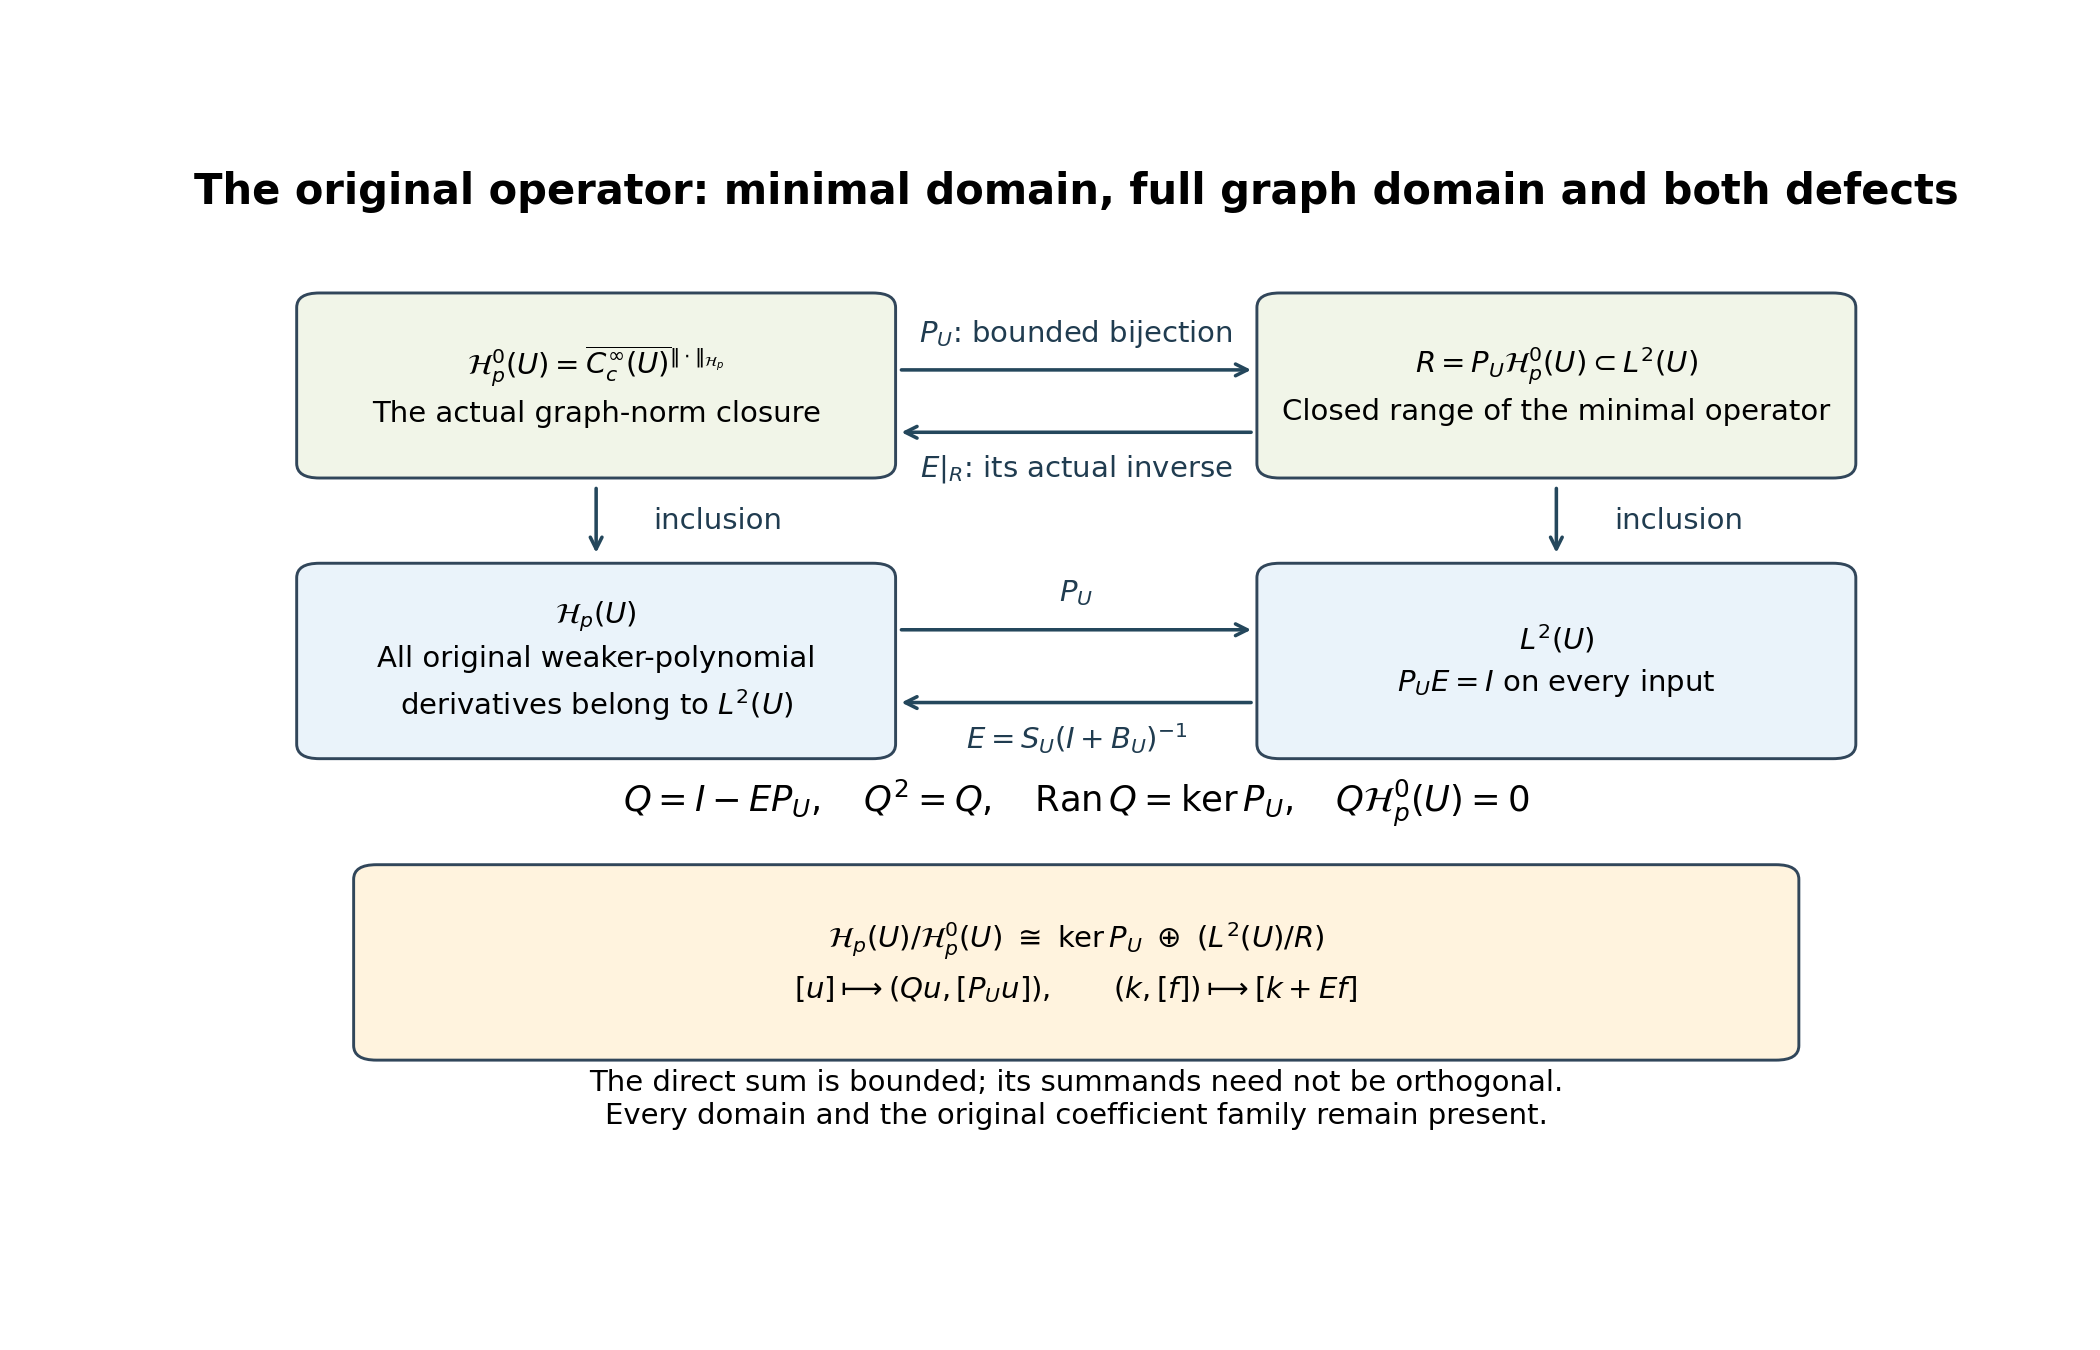
\includegraphics[width=.99\textwidth]{figures/graph_domain_defect_maps.png}
\caption{The original graph-domain maps and their two quotient factors. Proofs: GM8--GM11 and GM16--GM20.}
\end{figure}
\begin{figure}[htbp]\centering
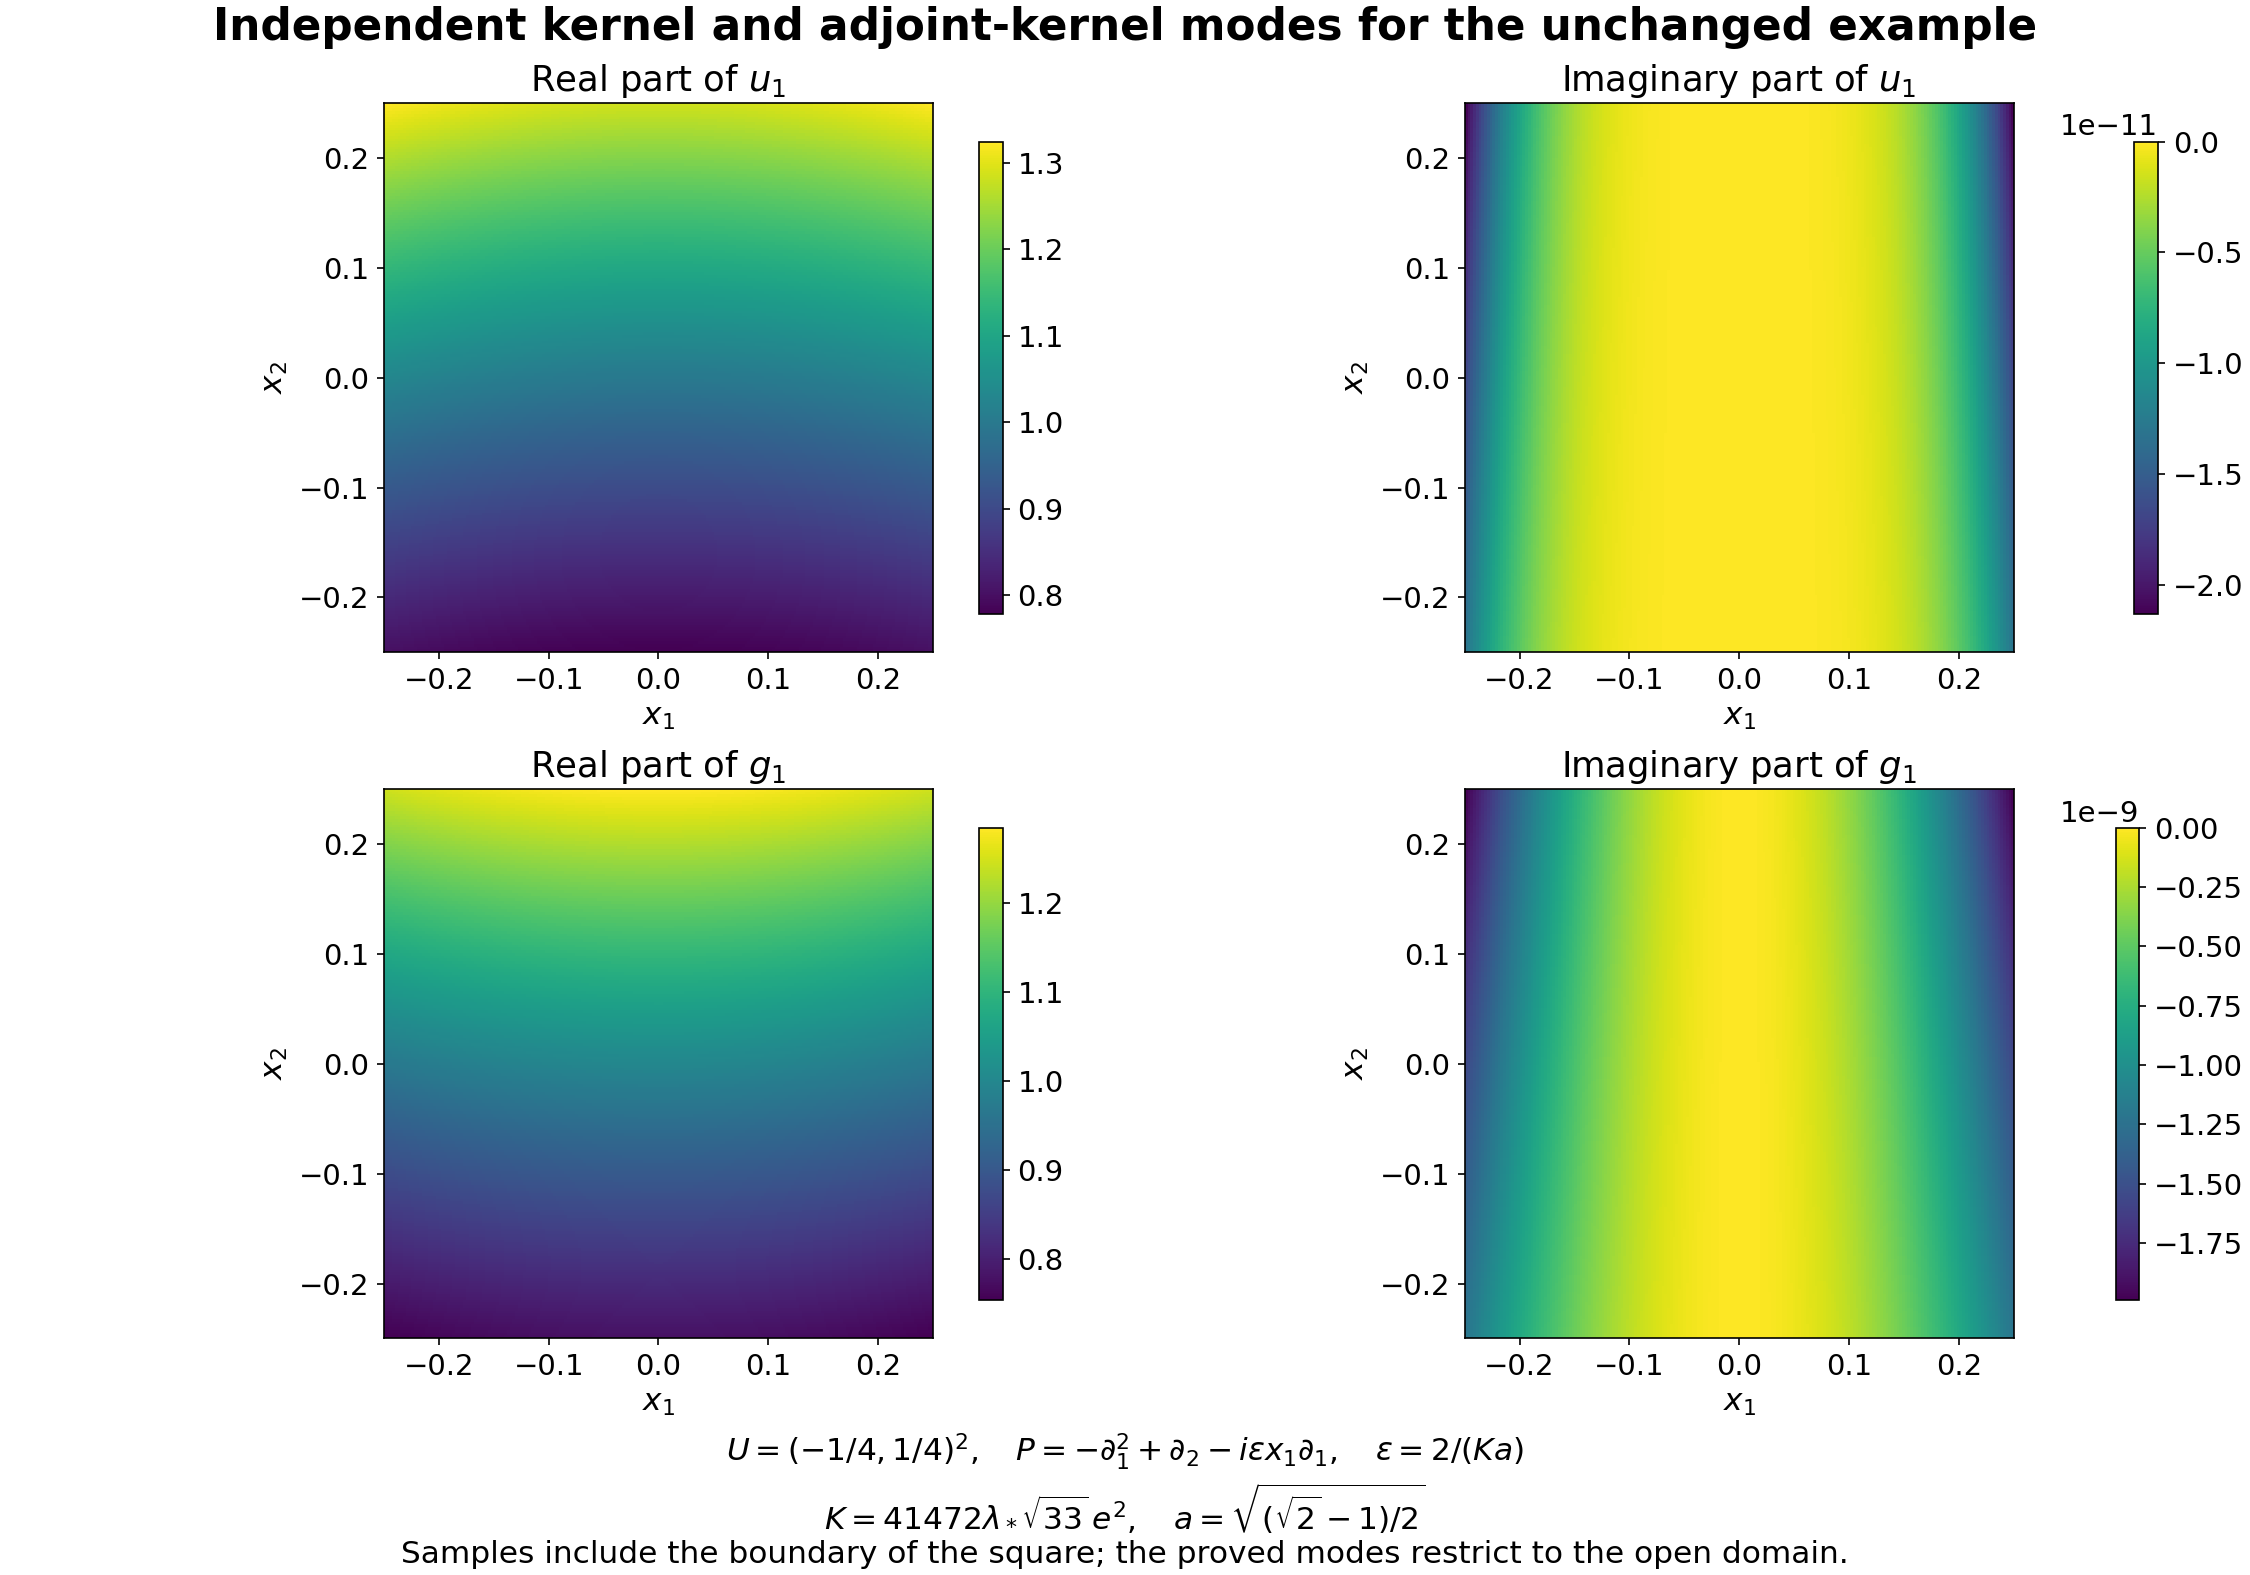
\includegraphics[width=.99\textwidth]{figures/original_coefficient_kernel_modes.png}
\caption{Kernel and adjoint-kernel samples for the unchanged example. Proofs: GM34, GM49 and GM50--GM52. Display rounding is not certified.}
\end{figure}

\end{document}
